%!TEX program = pdflatex
\documentclass[UTF8]{ctexart}
\usepackage{graphicx}
\usepackage{geometry}
\usepackage{multirow}
\usepackage{multicol}
\usepackage{amsmath}
\usepackage{amsthm}
\usepackage{amssymb}
\usepackage{bm}
\usepackage{amsfonts}
\usepackage{fancyhdr}
\usepackage{mathrsfs}
\usepackage{caption}
\usepackage{enumerate}
\usepackage{subfigure}
\usepackage{float}
\usepackage{circuitikz}
\usepackage{listings}
\geometry{papersize={21cm,29.7cm}}
\geometry{left=2.54cm,right=2.54cm,top=3.18cm,bottom=3.18cm}
\title{天气信息查询应用设计与实现}
\author{自12班\quad 阿拉帕提·吐尔逊\quad 2019010363}
\date{\today}
\pagestyle{fancy}
\lhead{\today}
\chead{}
\rhead{天气信息查询应用设计与实现}
\lfoot{Python程序设计}
\cfoot{\thepage}
\rfoot{智能传感与检测技术}
\renewcommand{\headrulewidth}{0.4pt}
\renewcommand{\headwidth}{\textwidth}
\renewcommand{\footrulewidth}{0pt}
\newtheorem*{theorem*}{定理}
\newtheorem{theorem}{定理}
\newtheorem*{corollary*}{推论}
\begin{document}
\maketitle
\lstset{language=python}
\lstset{
    numbers=left,
    numberstyle= \tiny,
    keywordstyle= \color{ blue!70},
    commentstyle= \color{red!50!green!50!blue!50},
    frame=shadowbox, % 阴影效果
    rulesepcolor= \color{ red!20!green!20!blue!20} ,
    escapeinside=\`\`, % 英文分号中可写入中文
    %xleftmargin=2em, aboveskip=1em,
    %framexleftmargin=2em
} 
\section{总体要求}

设计并实现一个天气信息查询应用,通过调用国内和国际天气API接口,
提供用户友好的图形用户界面,支持实时天气查询、图表展示和用户收藏功能。

\section{实现的功能}
\begin{itemize}
   \item 城市搜索:用户可以自行输入城市名称来搜索天气信息。
   \item 天气显示:
   
       (1)显示当日未来 24h (或者当日 24h)的天气状况,包括温度、湿度、风力风向等。
       
       (2) 展示所选城市的不同日期(包括今日和未来几日)对应的天气状况,包括温度、湿度、风力风向等。
   \item 数据更新:应用应能够定时从 API 获取最新数据,保持信息的实时性。
   \item 错误处理:当搜索不到相关城市或者API 服务不可用时,应用应能够给用户合适的反馈。
   \item 多地点保存:用户可以保存多个地点的天气信息,便于快速切换查看。
   \item 天气趋势图表:利用图表展示历史和预测的天气数据趋势,如温度曲线图等。
   \item 多语言支持:课根据用户偏好,切换应用中英文显示。
\end{itemize}

\section{模块讲解}
\subsection{依赖库}
\begin{itemize}
   \item requests:用来获取API返回的JSON数据。
   \item tkinter:用来创建图形用户界面。
   \item matplotlib:用来绘制天气趋势图。
   \item json:用来解析一个JSON数据文件,该文件是OpenWeatherMap提供的地理信息。
   \item datetime:用来获取当前时间。
   \item os:用来获取当前路径。
\end{itemize}

\subsection{API接口选择}
在本实验中,选择的国内API为高德地图天气API,
\textcolor{blue}{https://restapi.amap.com/v3/weather/weather\\Info?key={}\&city={}\&extensions=all},
包括国内的3241个省市区的天气信息供选择,天气信息的类别分别有白天/黑夜气温、湿度、风力风向、白天/黑夜天气情况等信息。
可以提供未来四日的天气预报。数据量简约,查询速度快,适合本实验的要求。

国际API为OpenWeatherMap API,
\textcolor{blue}{http://api.openweathermap.org/data/2.5/forecast?lat={lat}\&\\lon={lon}\&appid={appid}}。
包括国际上239个国家对应的城市和地区的天气信息,天气信息类别有气温、体感温度、风力风向、经纬度、压强、湿度等信息。
可以提供未来六日,间隔3小时的精确天气预报。数据量较大,查询速度较慢,但是提供了更多的天气信息。

\subsection{系统设计架构}
设计一个基于tkinter的图形用户界面,通过requests库调用API接口获取天气数据。
核心模块包括Weather(GlobalWeather)、WeatherGet(GlobalWeatherGet)、MyFavoriteCity以及WeatherGUI。
\begin{enumerate}[1.]
   \item Weather类和GlobalWeather类分别表示国内和国际城市的天气信息的数据结构,包括城市、日期、温度等信息。
         由于两种天气信息各有异同,因此没有设计继承类,而分别设计了两个类别。
   \item WeatherGet和GlobalWeatherGet类负责从API获取天气信息,并将其转化为Weather和Global\\Weather对象。
         \begin{itemize}
            \item WeatherGet类和GlobalWeatherGet类都包含\_\_init\_\_()、update\_weather()、add\_weather()、
                  get\_weather()等公有函数,负责将API返回的JSON数据转化为Weather和GlobalWeather对象,用来存储和查询。
         \end{itemize}
   \item MyFavoriteCity类用于管理用户收藏的城市和相应的天气信息。
         \begin{itemize}
            \item MyFavoriteCity类包含\_\_init\_\_()、add()、delete()、get\_classofcity()、get\_city\_codes()、
                  get\_\\city\_latlon()、get\_favor\_cityls()、\_\_del\_\_()等公有函数,负责管理用户收藏的城市和相应的天气信息。
            \item 在\_\_init\_\_()中,在类初始化时,从文件中读取用户以前收藏的城市信息,存储在列表中。在\_\_del\_\_()中,
                  在类销毁时,将用户收藏的城市信息写入文件。以便下次使用时读取。从而实现了数据的持久化。
         \end{itemize}
   \item WeatherGUI类是图形用户界面的核心,负责展示天气信息、图表绘制和用户交互。
         \begin{itemize}
            \item WeatherGUI类包含\_\_init\_\_()、update\_weather()、create\_menu()、national()、international()、show\_favorite()、chinese()、english()等主要的公有函数。
            \item update\_weather()函数负责定时从API获取天气信息,并更新界面上的天气信息。保证数据的实时性。
            \item create\_menu()函数负责创建菜单栏,包括国内/国际天气查询、收藏列表、语言切换等功能。
            \item national()函数创建国内天气查询窗口,调用WeatherGet类获取天气信息,并在界面上展示。
            \item international()函数创建国际天气查询窗口,调用GlobalWeatherGet类获取天气信息,并在界面上展示。
            \item show\_favorite()函数创建收藏列表窗口,调用MyFavoriteCity类获取用户收藏的城市信息和天气信息,并在界面上展示。
            \item chinese()和english()函数分别切换界面语言为中文和英文。
         \end{itemize}
\end{enumerate}

\subsection{核心模块详解}

\begin{enumerate}
   \item \textbf{national()}

         该函数主要负责创建国内天气查询窗口的所有组建,并根据用户的交互,调用相关函数显示天气信息。

         \textbf{城市和日期下拉框回调函数}
         \begin{itemize}
            \item city\_combobox\_selected()函数和date\_combobox\_selected()函数分别是界面中城市下拉框和日期下拉框的回调函数,
                  前者将调用WeatherGet类获取天气信息,而后使用update\_\\weather\_info()函数更新界面天气信息,
                  后者将直接调用update\_weather\_info()函数更新天气信息。
                  \begin{figure}[H]
                     \centering
                     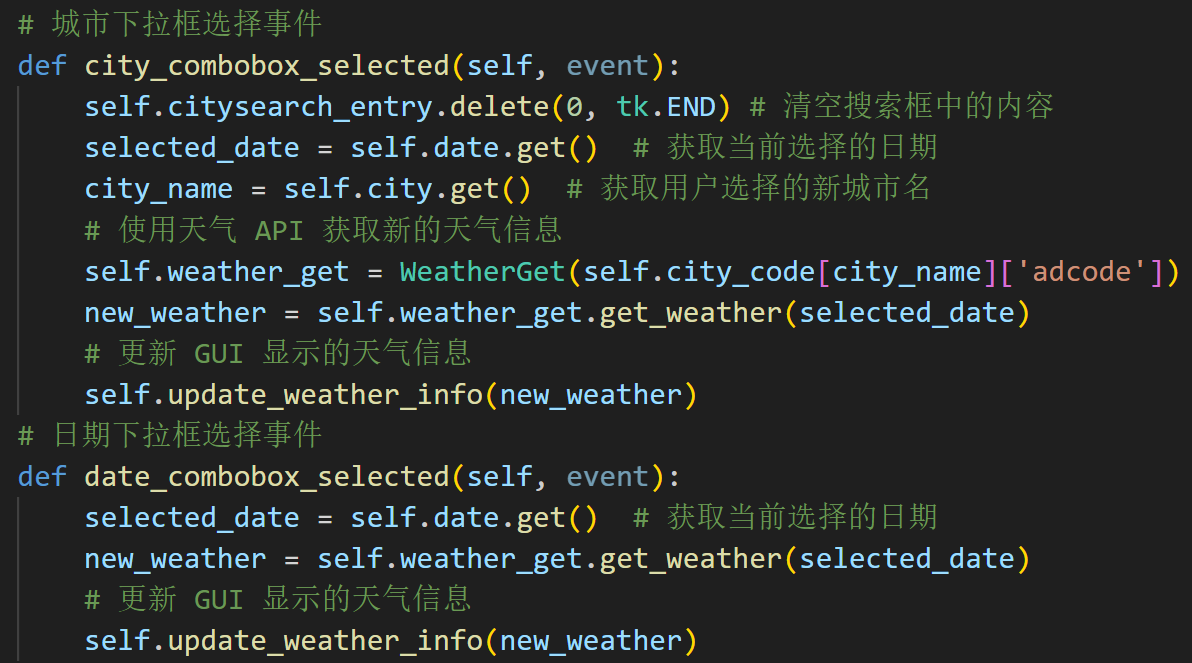
\includegraphics[width=0.8\textwidth]{pic1.png}
                     \caption{city\_combobox\_selected()函数和date\_combobox\_selected()函数}
                  \end{figure}
            \item update\_weather\_info()函数负责更新界面上的天气信息,包括实时温度、湿度、风向等。
            \begin{figure}[H]
               \centering
               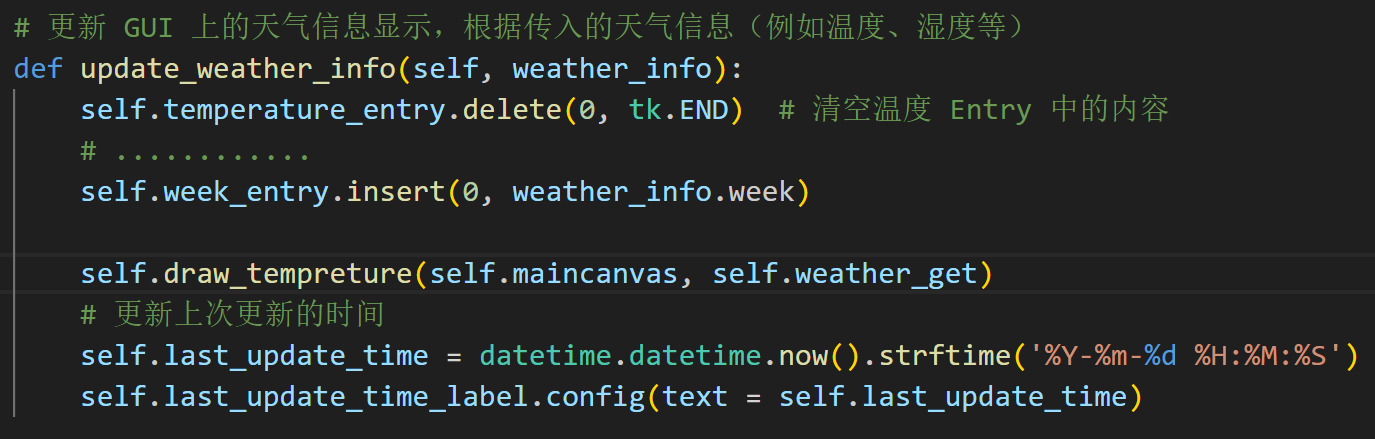
\includegraphics[width=0.8\textwidth]{pic2.png}
               \caption{update\_weather\_info()函数}
            \end{figure}
         \end{itemize}
         \textbf{搜索框回调函数}
         \begin{itemize}
            \item search()函数将实时根据用户输入查找库中的可查询的城市信息,并把可能的城市信息在搜索显示框中显示。
            \begin{figure}[H]
               \centering
               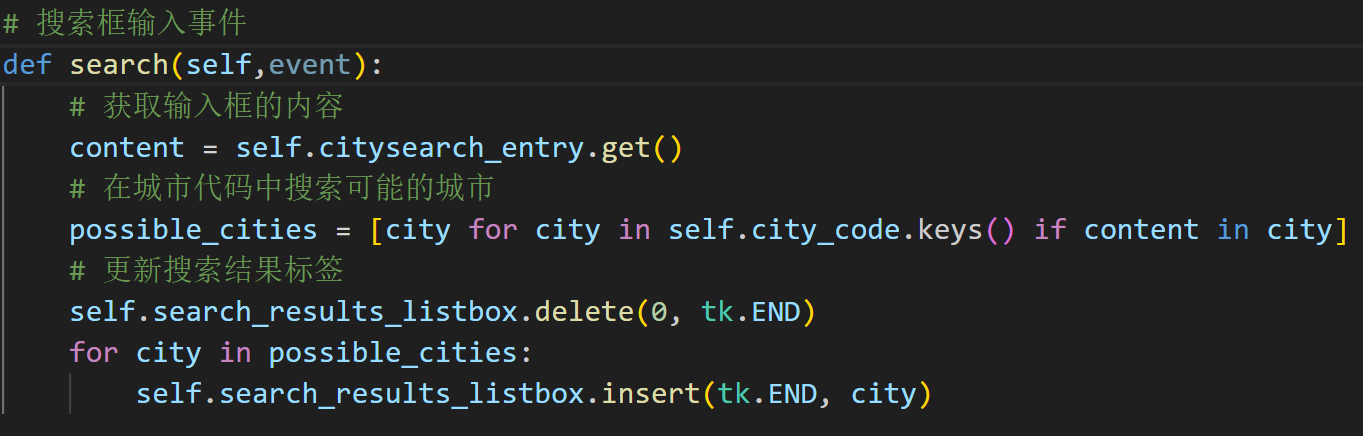
\includegraphics[width=0.8\textwidth]{pic3.png}
               \caption{search()函数}
            \end{figure}
            \item on\_select()函数是搜索显示框的回调函数,将用户选择的城市信息填入搜索框中。
            \begin{figure}[H]
               \centering
               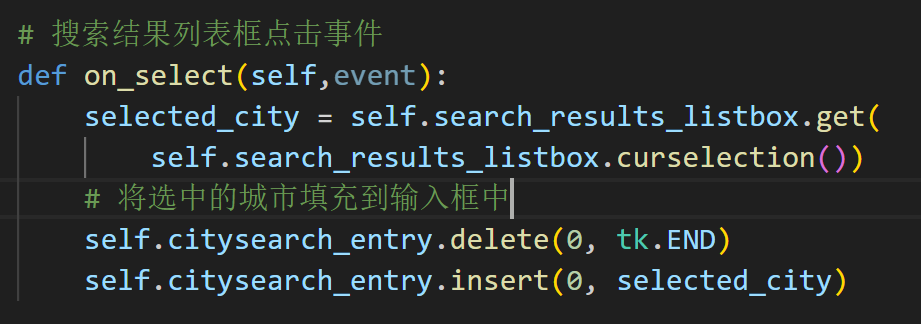
\includegraphics[width=0.8\textwidth]{pic4.png}
               \caption{on\_select()函数}
            \end{figure}
            \item citysearch\_button\_clicked()函数是搜索按钮的回调函数,将根据用户输入的城市信息调用WeatherGet类获取天气信息。
            \begin{figure}[H]
               \centering
               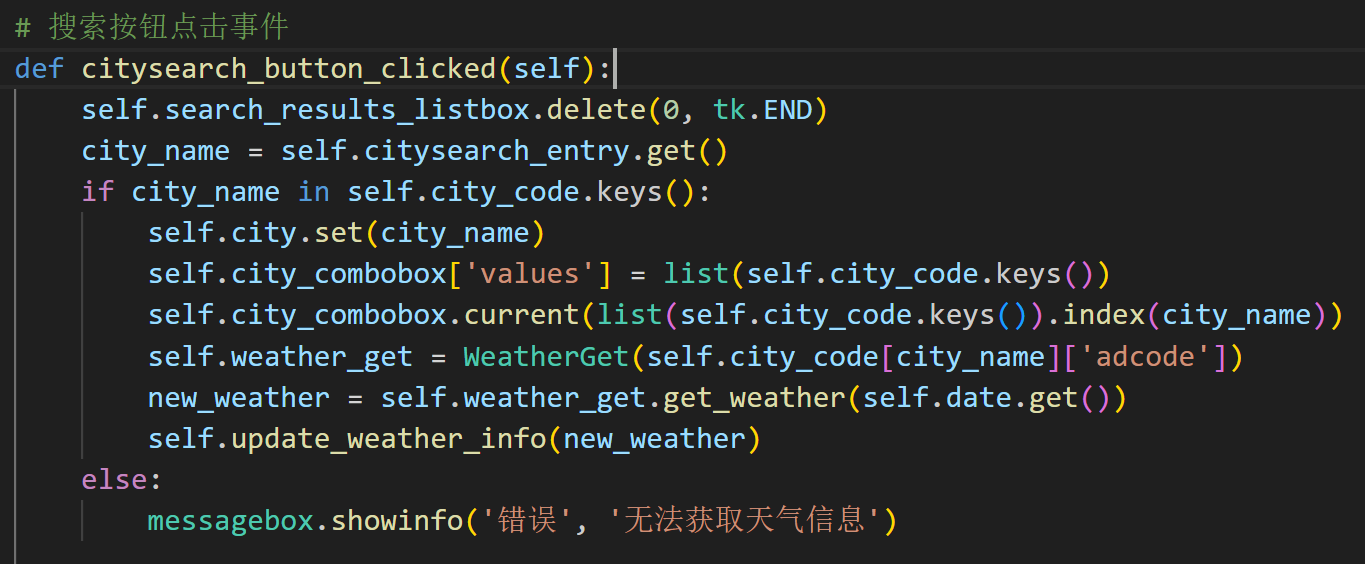
\includegraphics[width=0.8\textwidth]{pic5.png}
               \caption{citysearch\_button\_clicked()函数}
            \end{figure}
         \end{itemize}
         \textbf{天气趋势图}
         \begin{itemize}
            \item draw\_tempreture()函数负责根据已获取的天气信息绘制未来几天的天气趋势图,并把图片嵌入到窗口中。
            \begin{figure}[H]
               \centering
               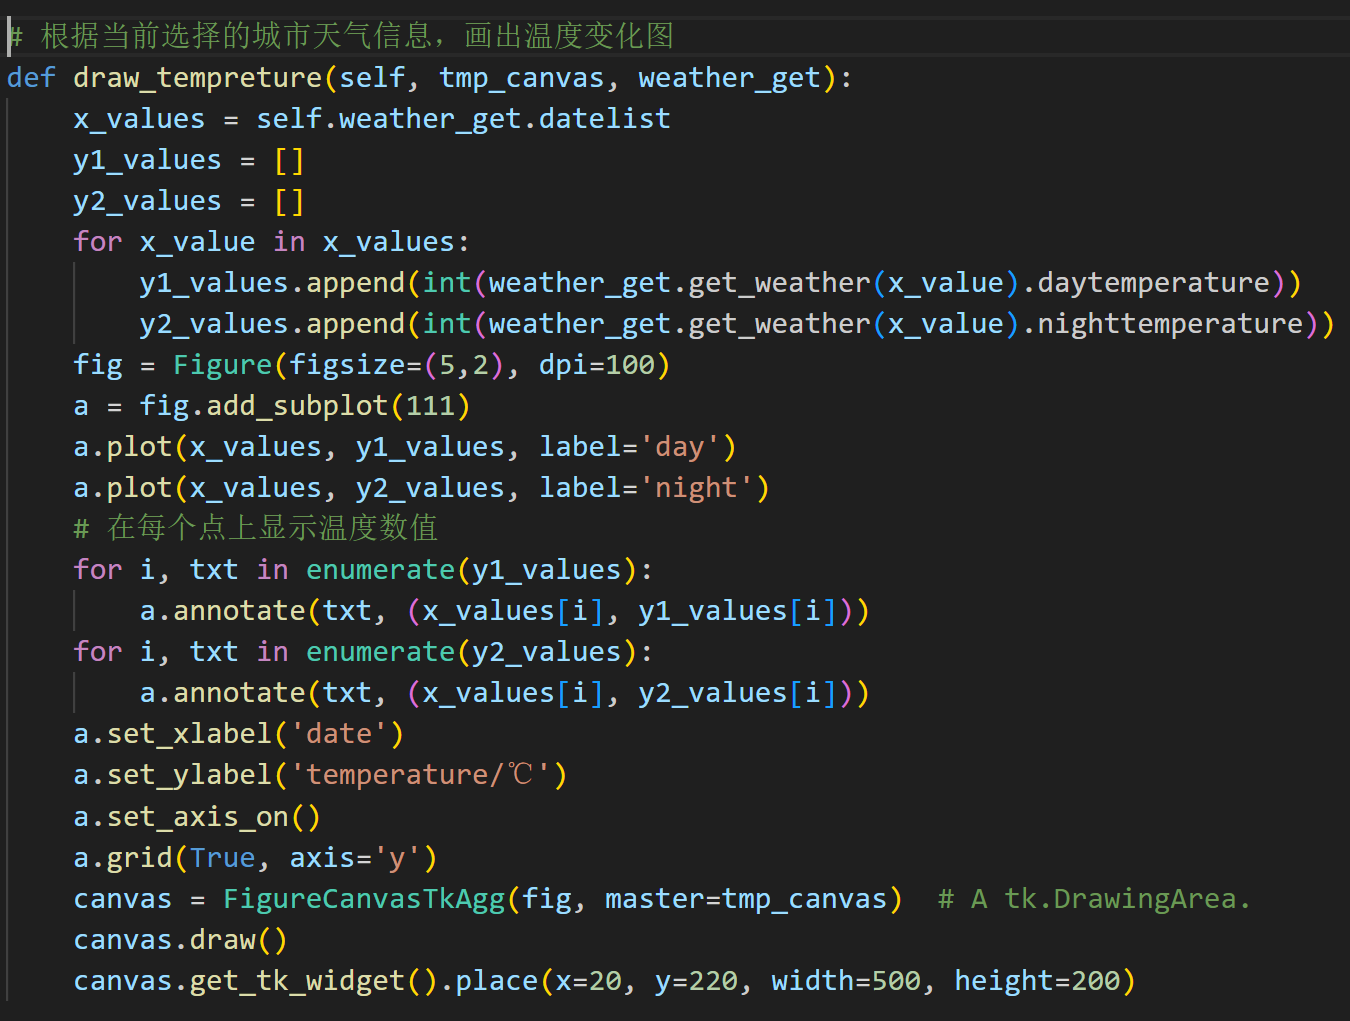
\includegraphics[width=0.8\textwidth]{pic6.png}
               \caption{draw\_tempreture()函数}
            \end{figure}
         \end{itemize}

   
   \item \textbf{international()}
   
   该函数创建国际天气查询窗口的所有组建,并根据用户的交互,调用相关函数显示天气信息。

   \textbf{国家、城市、时间下拉框回调函数}
   \begin{itemize}
      \item country\_combobox\_selected()函数是国家下拉框的回调函数,将更新城市下拉框城市列表,而后调用GlobalWeatherGet类获取天气信息。
      \begin{figure}[H]
         \centering
         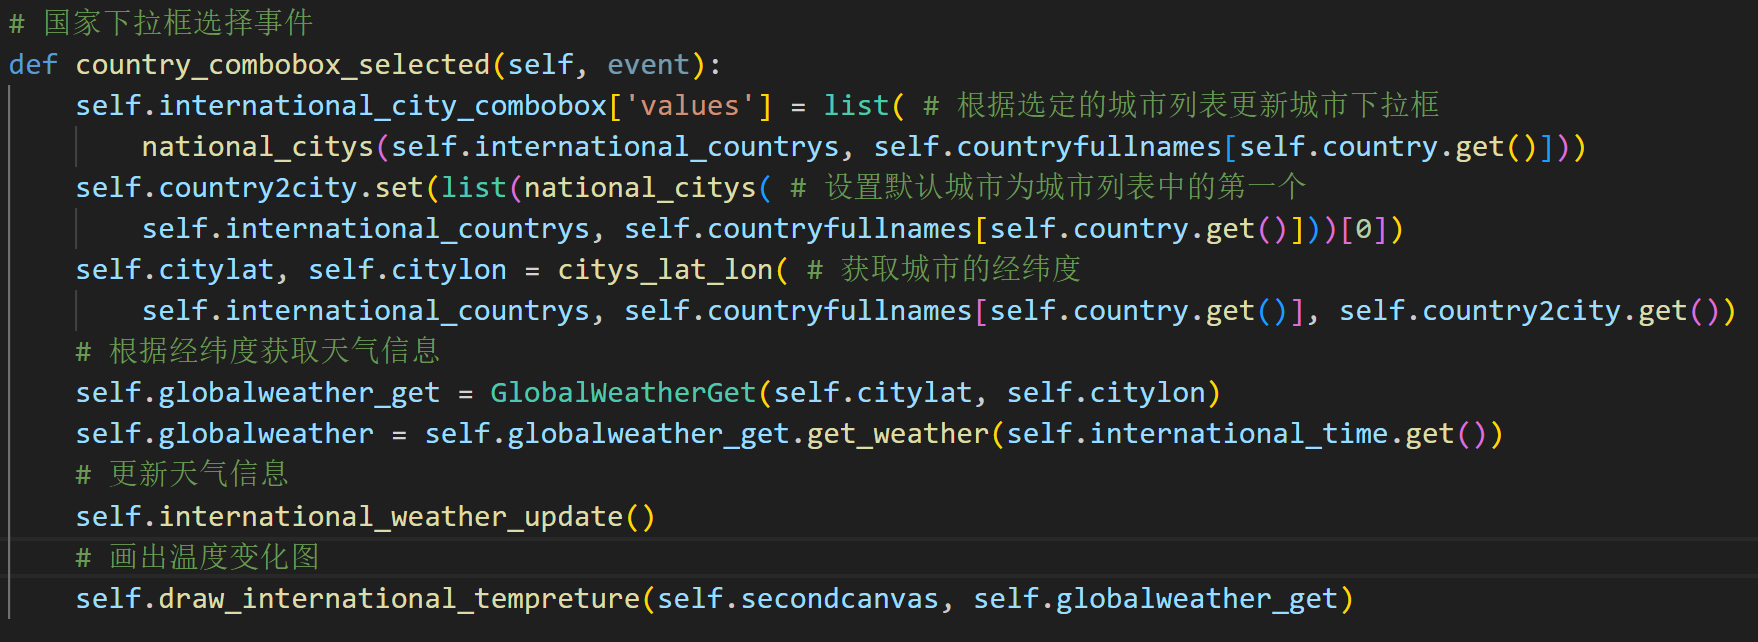
\includegraphics[width=0.8\textwidth]{pica.png}
         \caption{country\_combobox\_selected()函数}
      \end{figure}
      \item city\_combobox\_selected()函数是城市下拉框的回调的函数,将根据已选的国家、城市调用GlobalWeatherGet类获取天气信息。
      \begin{figure}[H]
         \centering
         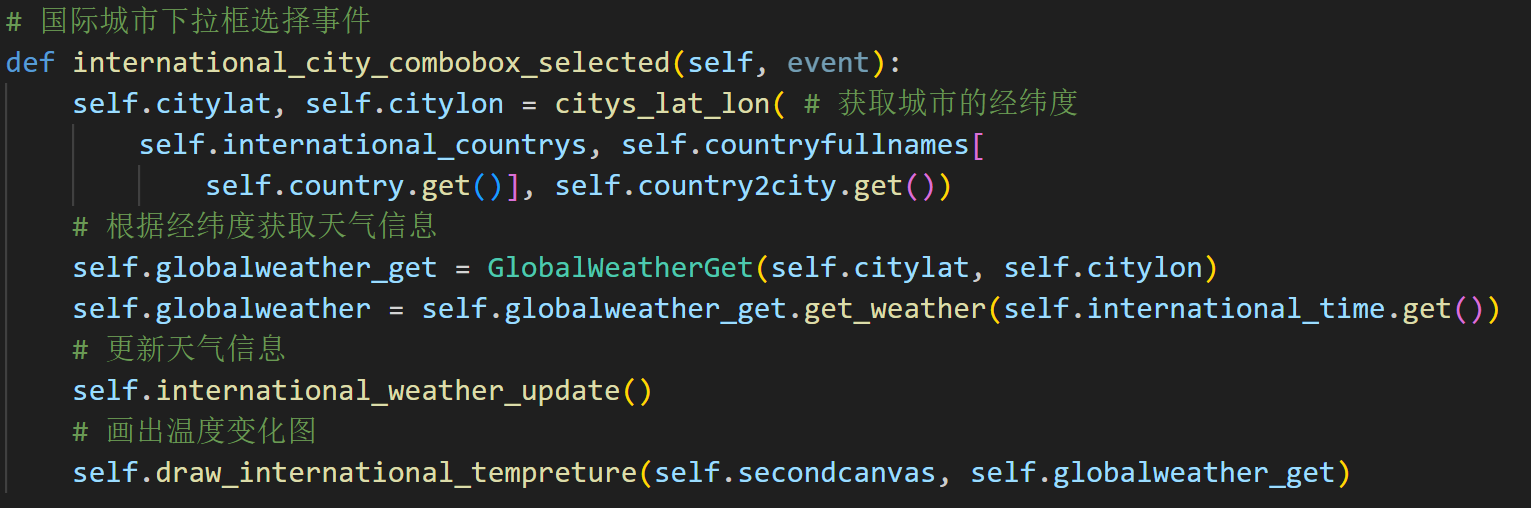
\includegraphics[width=0.8\textwidth]{picb.png}
         \caption{city\_combobox\_selected()函数}
      \end{figure}
      \item international\_time\_combobox\_selected()是日期下拉框的回调函数,将根据已选的日期已获取的天气信息查找并更新天气信息。
      \begin{figure}[H]
         \centering
         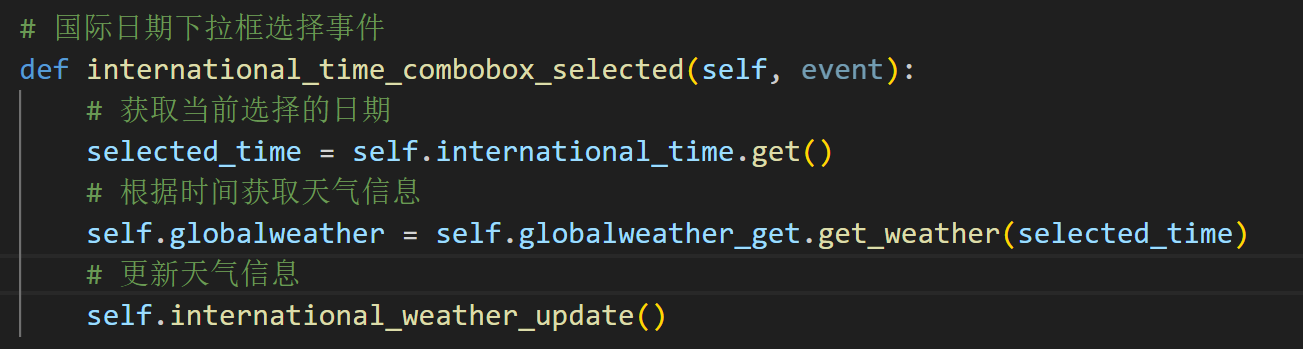
\includegraphics[width=0.8\textwidth]{picc.png}
         \caption{international\_time\_combobox\_selected()函数}
      \end{figure}
      \item international\_weather\_update()函数负责更新界面上的天气信息,包括温度、湿度、风向等。
      \begin{figure}[H]
         \centering
         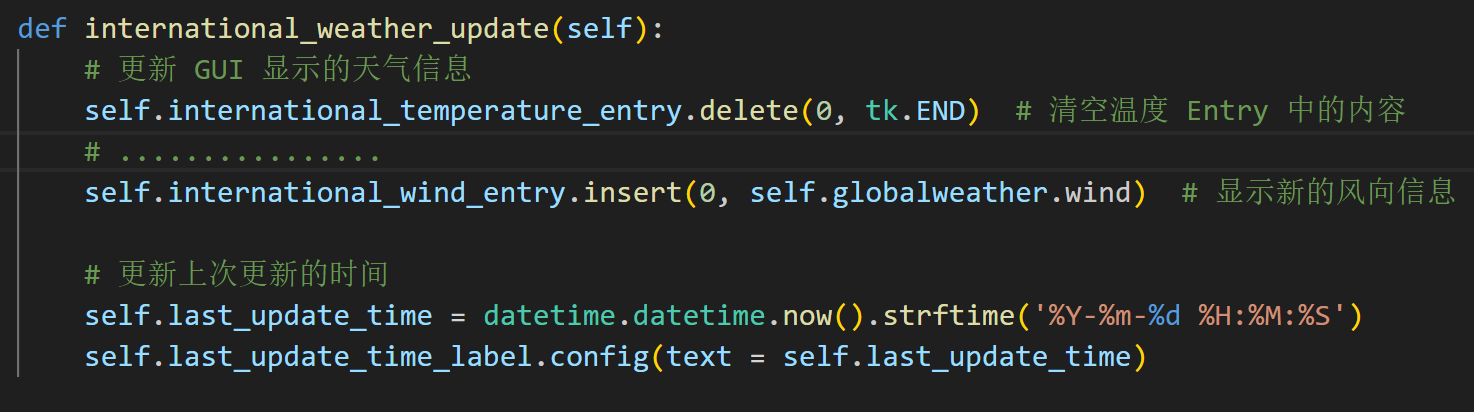
\includegraphics[width=0.8\textwidth]{picd.png}
         \caption{international\_weather\_update()函数}
      \end{figure}
   \end{itemize}
   \textbf{天气趋势图}
   \begin{itemize}
      \item draw\_internationa\_tempreture()函数负责根据已获取的天气信息绘制未来几天的天气趋势图,并把图片嵌入到窗口中。
      \begin{figure}[H]
         \centering
         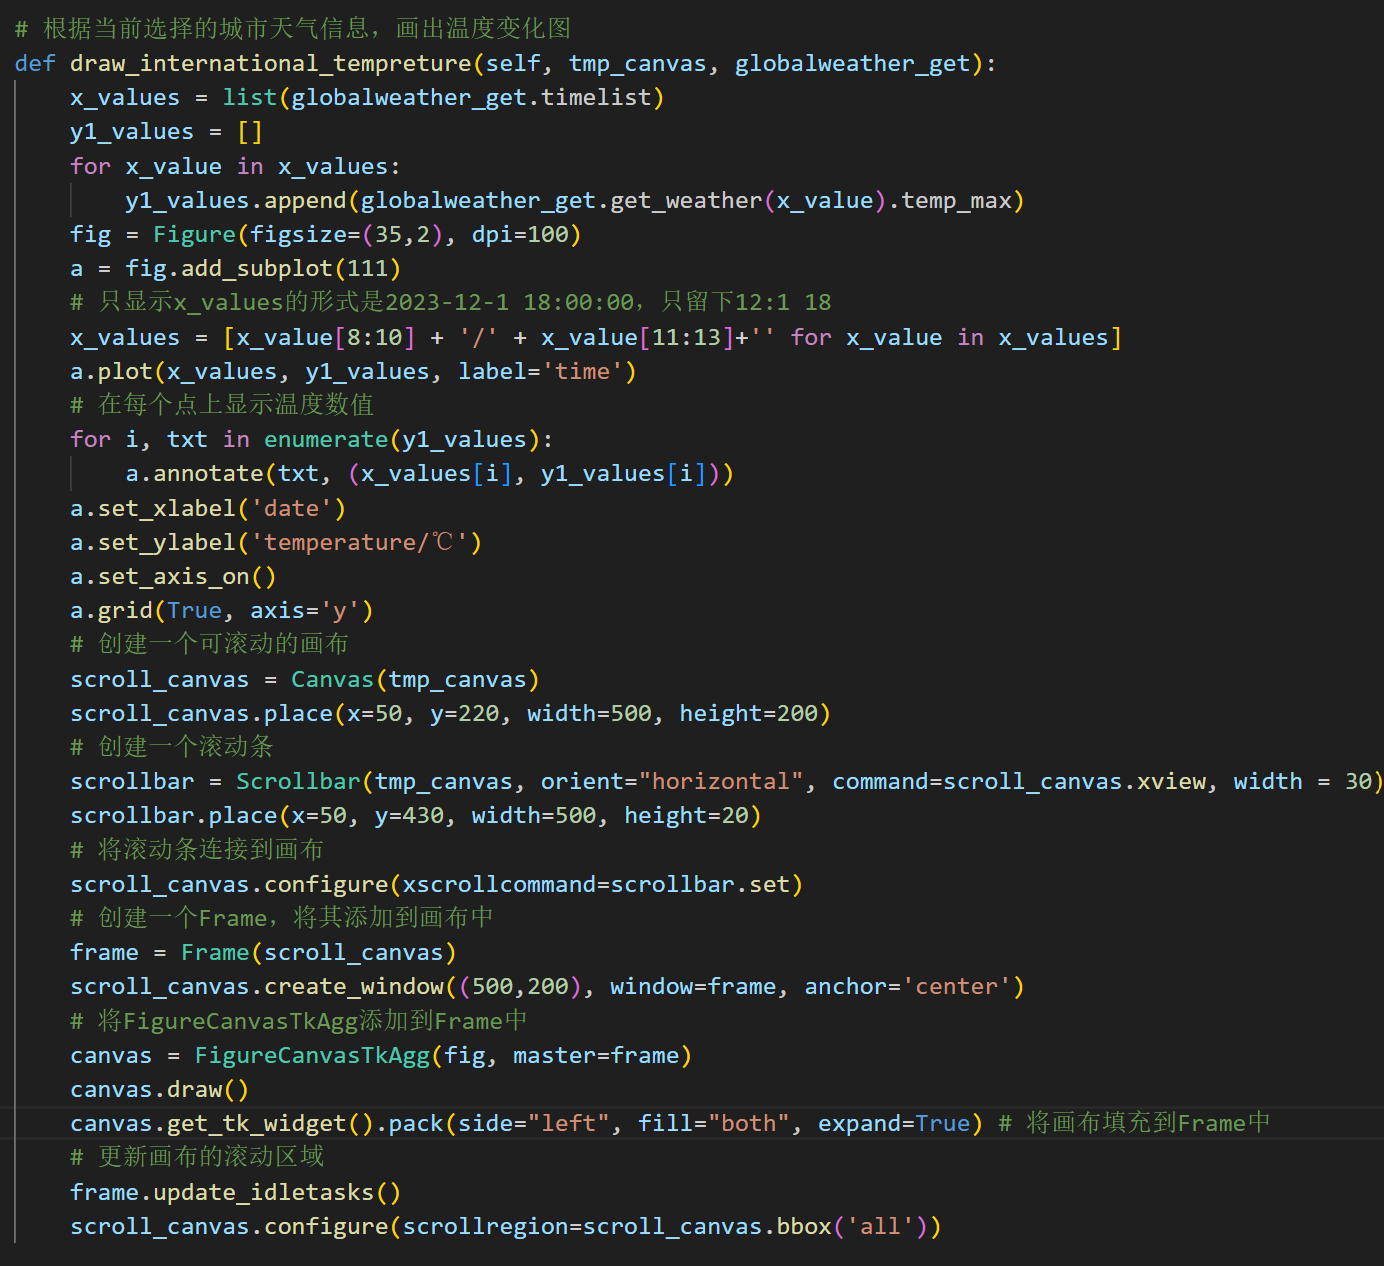
\includegraphics[width=0.8\textwidth]{pice.png}
         \caption{draw\_international\_tempreture()函数}
      \end{figure}
   \end{itemize}
   
   \item \textbf{收藏夹}
   \begin{itemize}
      \item show\_favorite()函数创建收藏列表窗口,调用MyFavoriteCity类获取用户收藏的城市信息和天气信息,并在界面上展示。
      \begin{figure}[H]
         \centering
         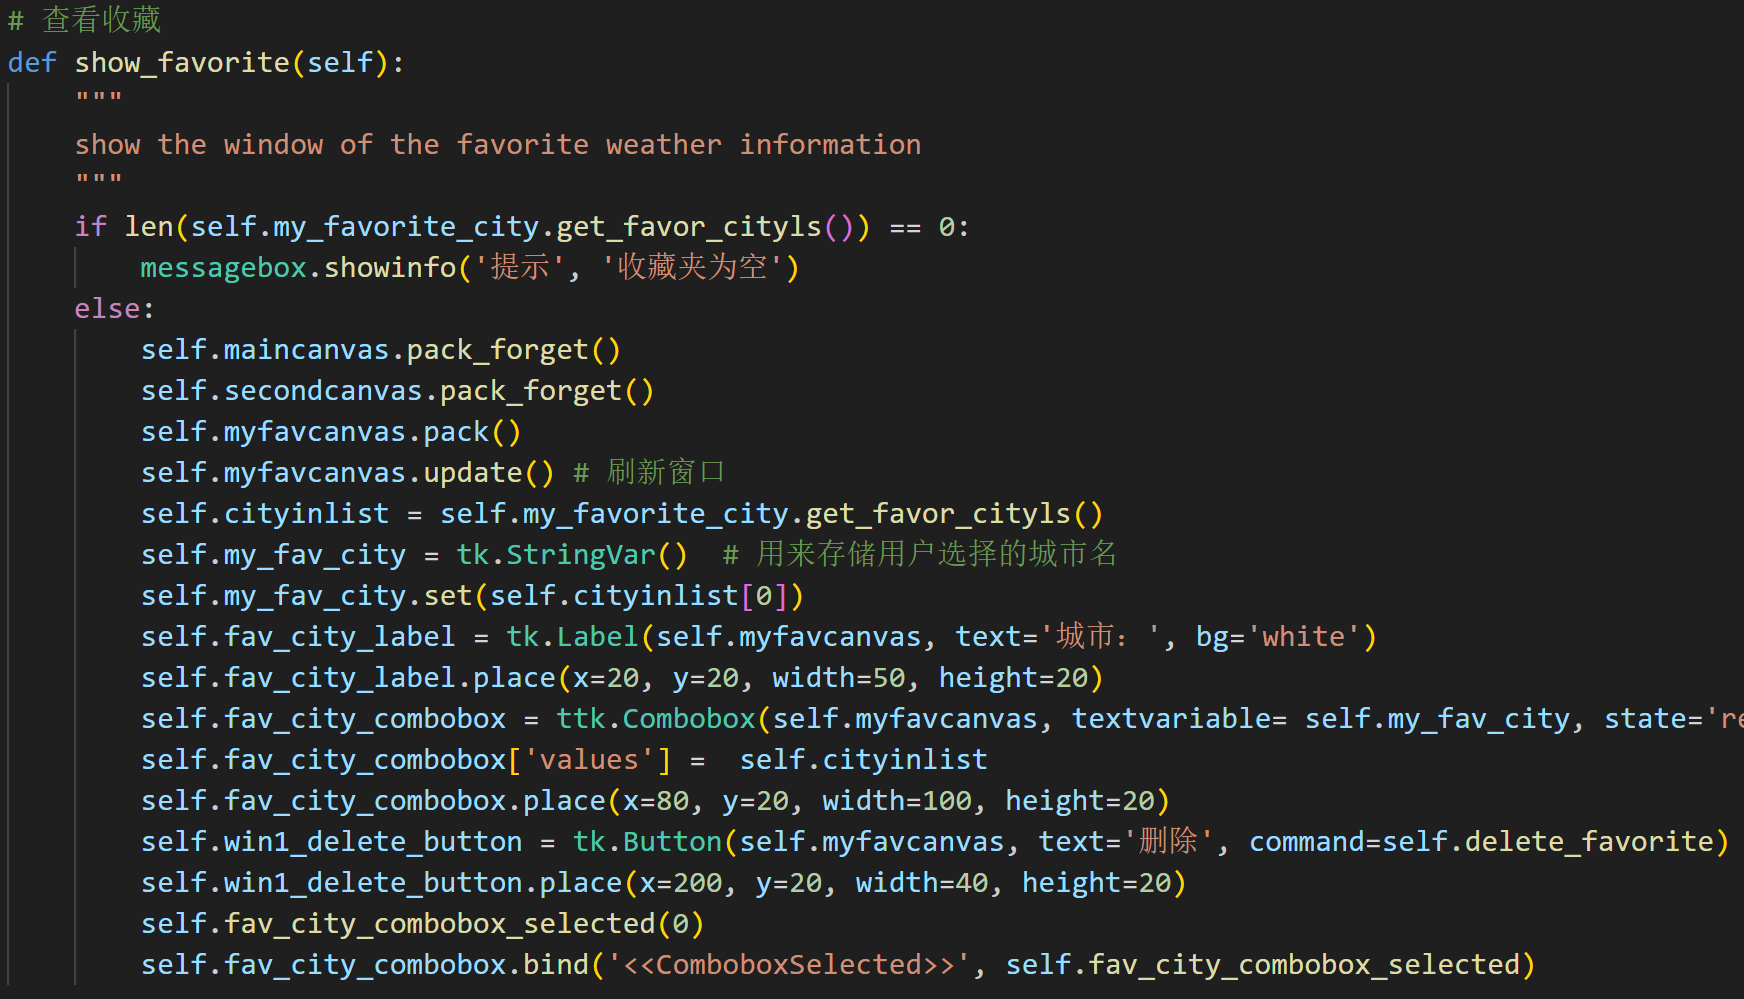
\includegraphics[width=0.8\textwidth]{pica1.png}
         \caption{show\_favorite()函数}
      \end{figure}
      \item add\_favorite()函数是添加收藏按钮的回调函数,在国内和国际天气信息显示界面时,将收藏的城市信息存储到列表中。
      \begin{figure}[H]
         \centering
         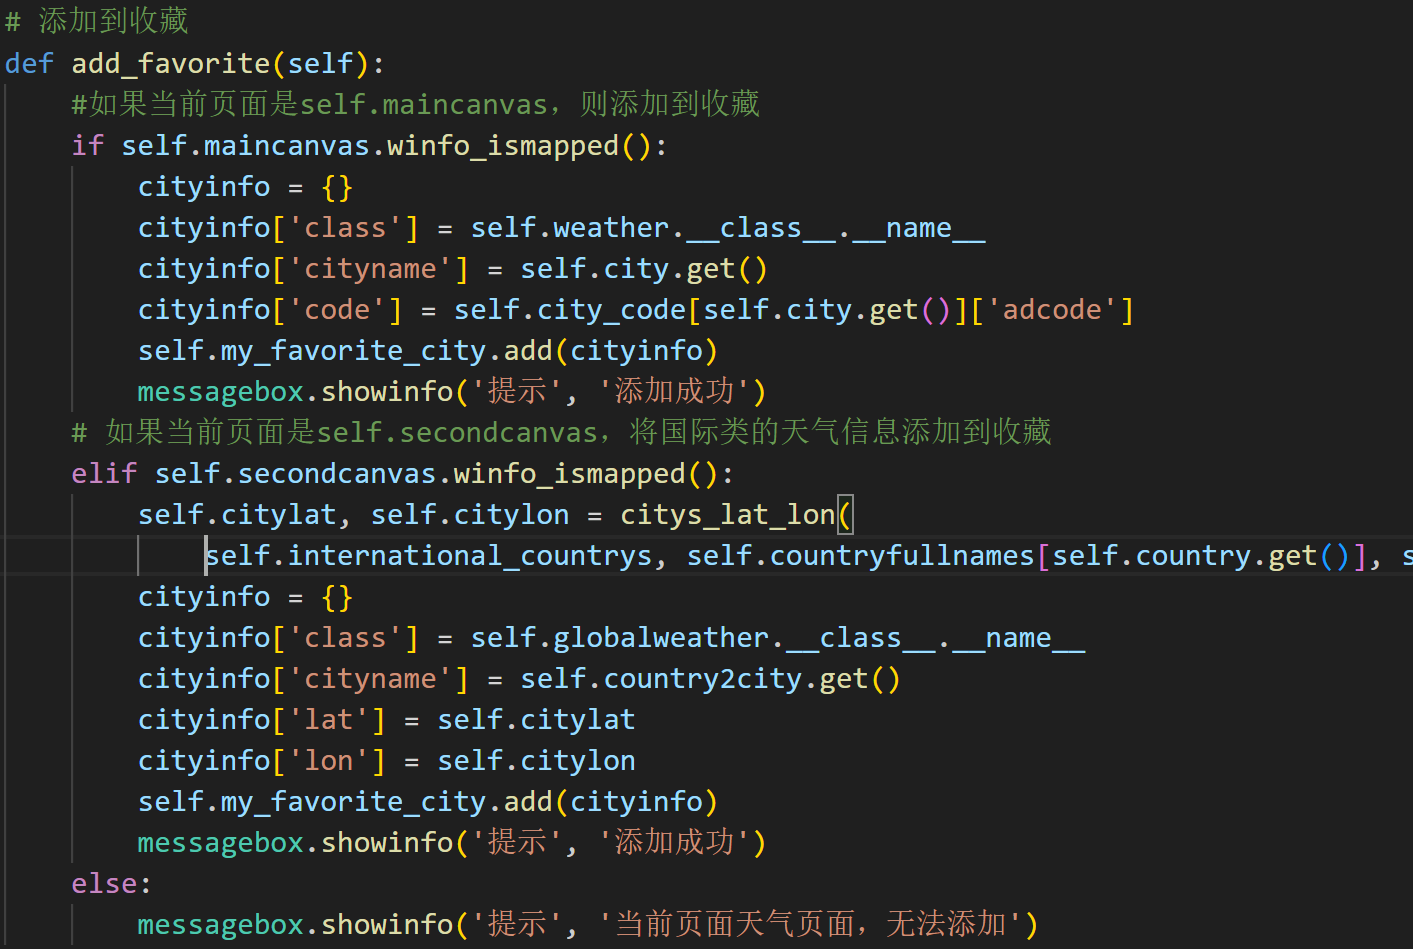
\includegraphics[width=0.8\textwidth]{pica2.png}
         \caption{add\_favorite()函数}
      \end{figure}
      \item delete\_favorite()函数是删除收藏按钮的回调函数,在收藏列表界面时,将收藏的城市信息从列表中删除。
      \begin{figure}[H]
         \centering
         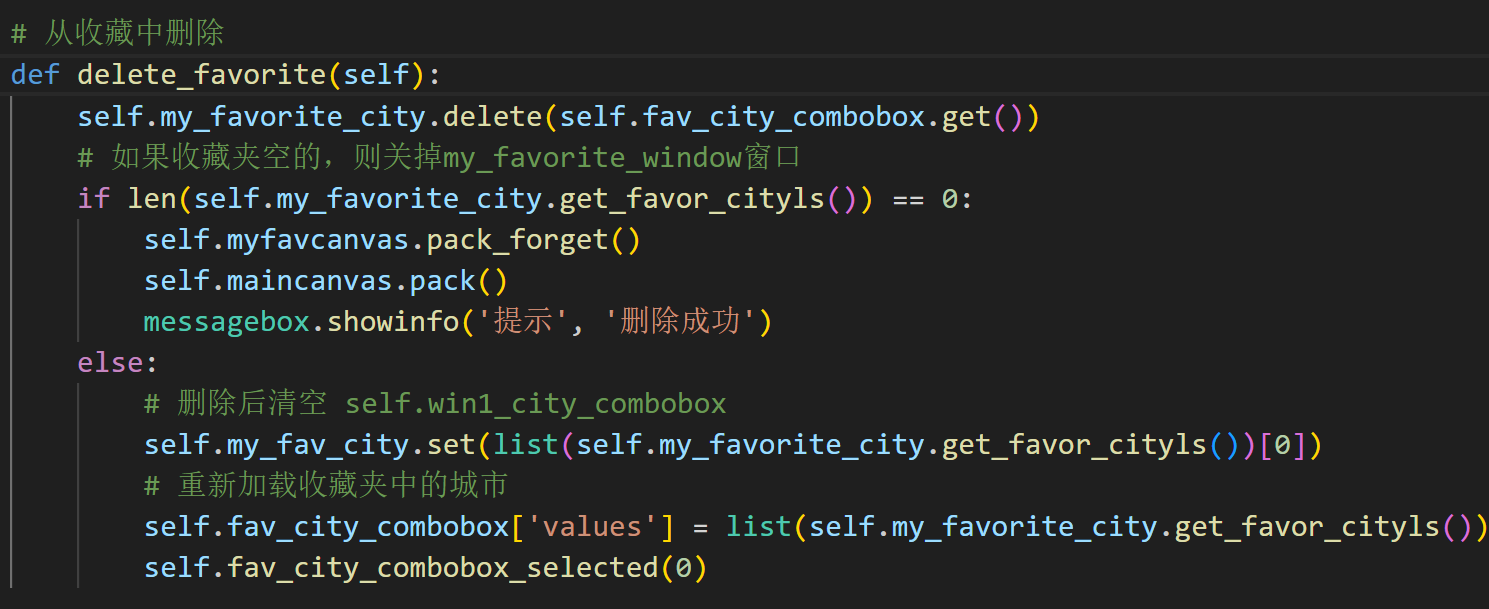
\includegraphics[width=0.8\textwidth]{pica3.png}
         \caption{delete\_favorite()函数}
      \end{figure}
      \item fav\_city\_combobox\_selected()函数是收藏列表界面城市下拉框的回调函数,将根据已选的城市信息从API获取天气信息并更新界面。
      \begin{figure}[H]
         \centering
         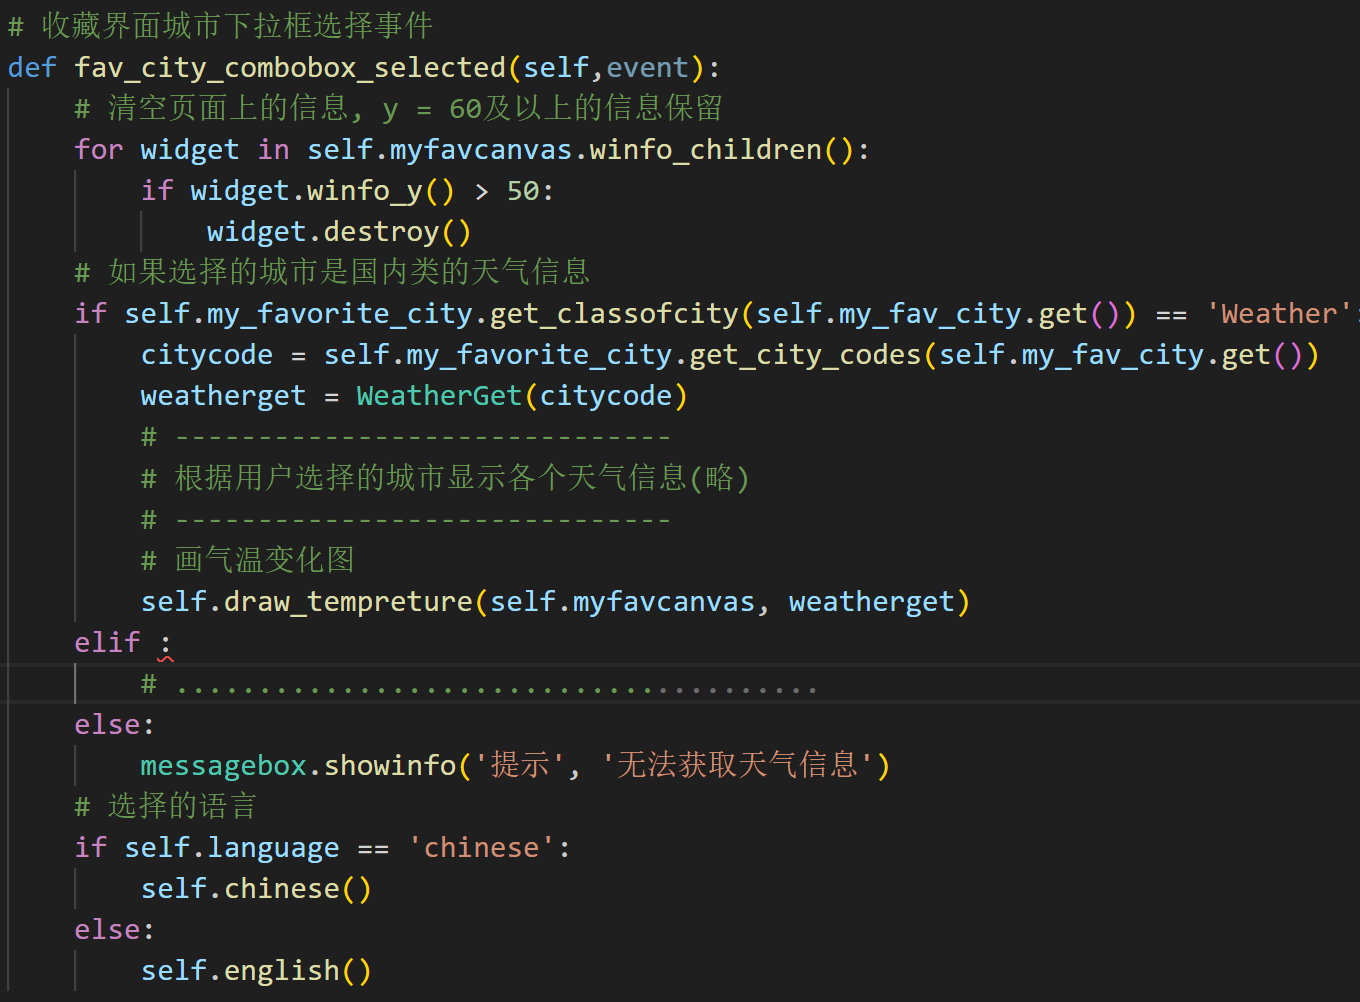
\includegraphics[width=0.8\textwidth]{pica4.png}
         \caption{fav\_city\_combobox\_selected()函数}
      \end{figure}
   \end{itemize}


\end{enumerate}

\subsection{交互流程}
\begin{enumerate}
   \item 菜单栏
   \begin{itemize}
      \item 收藏:包含“添加至收藏和查看收藏”。选择添加至收藏可将当前城市添加至收藏列表,选择查看收藏可查看收藏列表。
      \item 语言/language:选择中文或英文。选择中文将切换界面语言为中文,选择英文将切换界面语言为英文。
      \item 国内/国际:选择国内将切换到国内天气查询界面,选择国际将切换到国际天气查询界面。
      \begin{figure}[H]
         \centering
         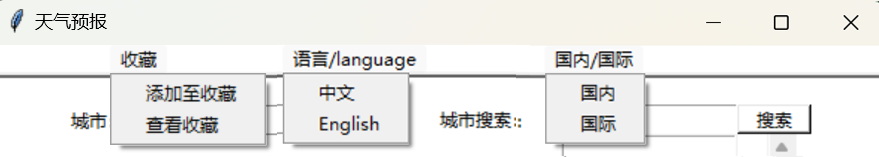
\includegraphics[width=0.8\textwidth]{picb1.png}
         \caption{菜单栏}
      \end{figure}
   \end{itemize}
   \item 国内天气查询:
         \begin{itemize}
            \item 用户打开应用,默认显示北京市天气信息
            \item 在城市下拉框中选择城市或者在日期下拉框选择日期均能更新天气信息。
            \item 如果想搜索指定信息可在搜索框中输入城市信息,(搜索显示框将显示匹配的城市,点击可将其填入搜索框中),点击搜索按钮,即可更新天气信息。
            \item 显示查询结果,包括实时温度、湿度、风向等。
            \item 下方显示未来几天的天气趋势图和最近一次的更新时间。
            \begin{figure}[H]
               \centering
               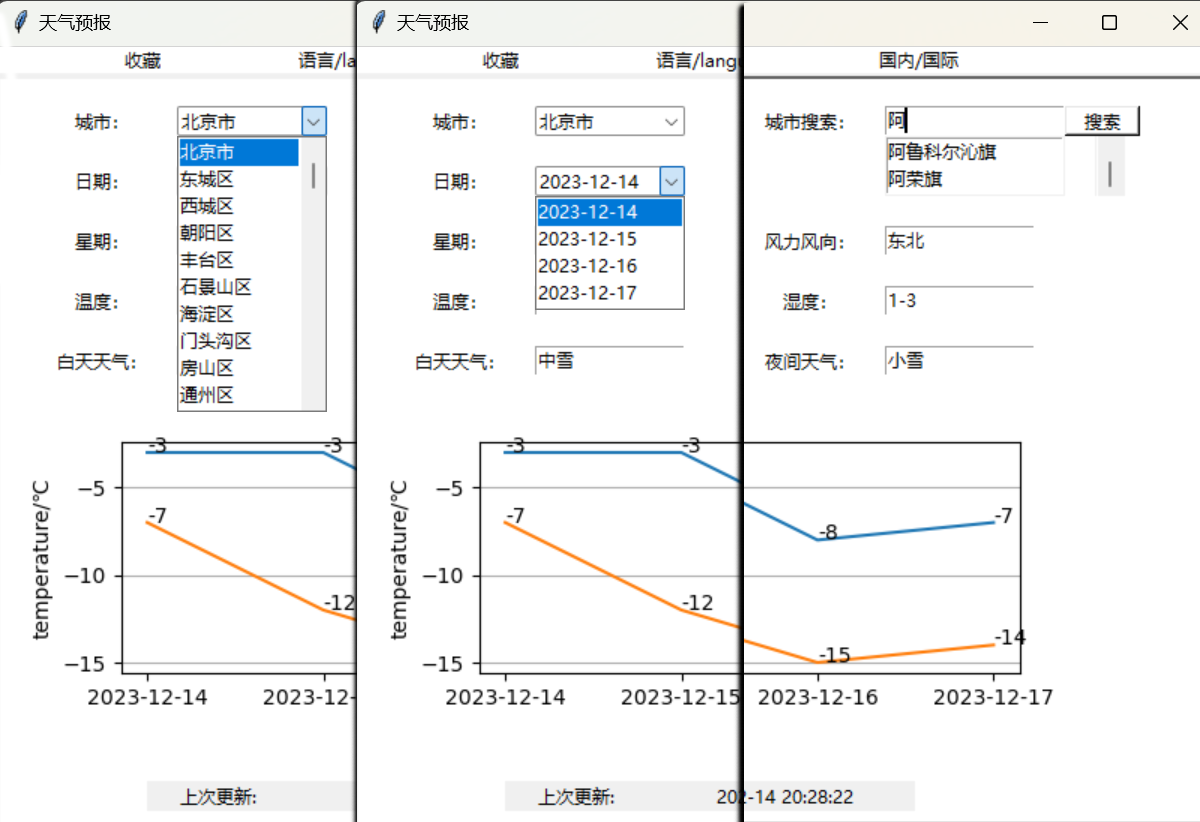
\includegraphics[width=0.8\textwidth]{picb2.png}
               \caption{国内天气查询}
            \end{figure}
         \end{itemize}
   \item 国际天气查询:
         \begin{itemize}
            \item 点击菜单栏国际按钮,切换到国际天气查询界面。默认显示China,Beijing的天气信息。
            \item 在国家下拉框中选择国家,在城市下拉框选择城市,在时间下拉框选择时间均能更新界面天气信息。
            \item 界面显示查询结果,包括温度、湿度、风向等。
            \item 下方显示未来几天的天气趋势图(可通过滑条拖动查看)和最近一次的更新时间
            \begin{figure}[H]
               \centering
               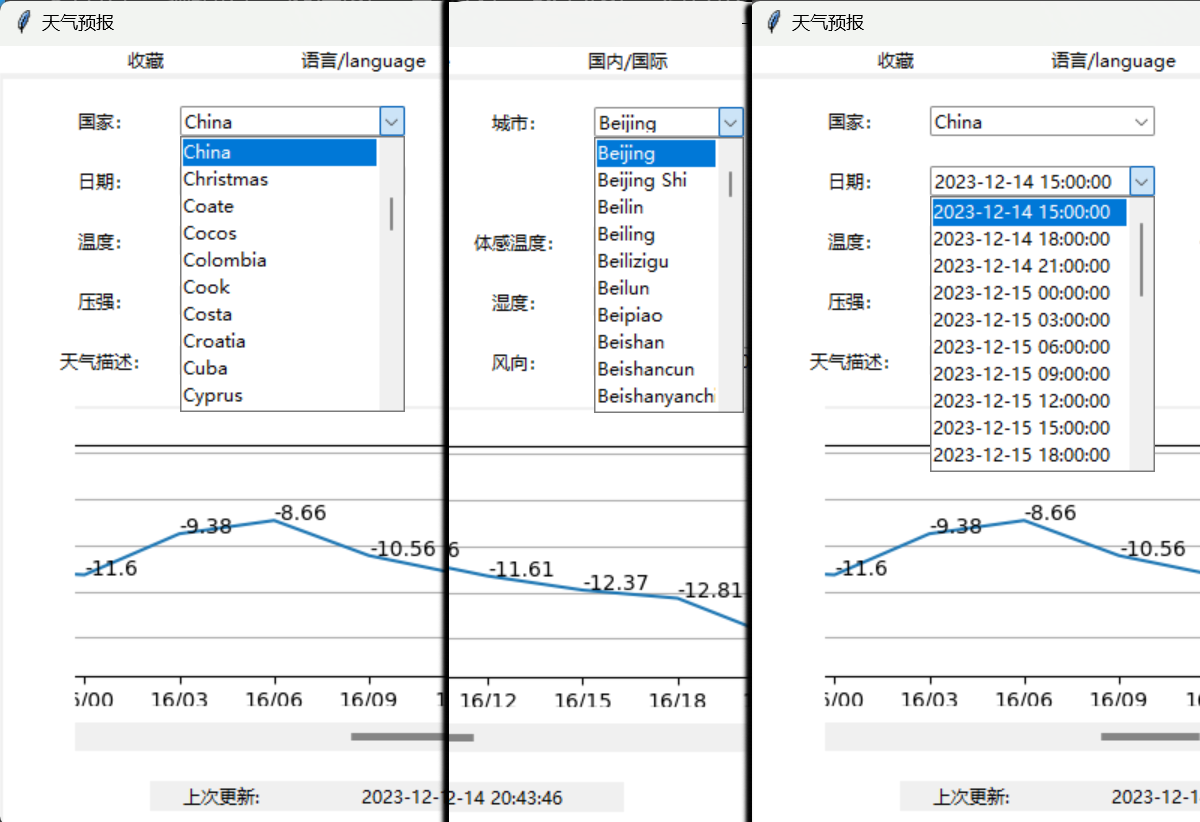
\includegraphics[width=0.8\textwidth]{picb3.png}
               \caption{国际天气查询}
            \end{figure}
         \end{itemize}
   \item 查看收藏列表:
         \begin{itemize}
            \item 用户点击“添加收藏”按钮,将把当前城市添加至收藏列表。
            \item 用户点击“收藏列表”按钮,若已有收藏城市,将显示收藏列表界面。否则提示用户收藏列表为空。
            \item 收藏列表界面显示用户收藏的城市列表,在城市下拉框选择城市,可更新界面天气信息。
            \item 用户点击“删除”按钮将把当前城市从收藏列表中删除。
            \item 界面显示查询结果,包括温度、湿度、风向等。
            \item 下方显示未来几天的天气趋势图(国际城市的可通过滑条拖动查看)。
            \begin{figure}[H]
               \centering
               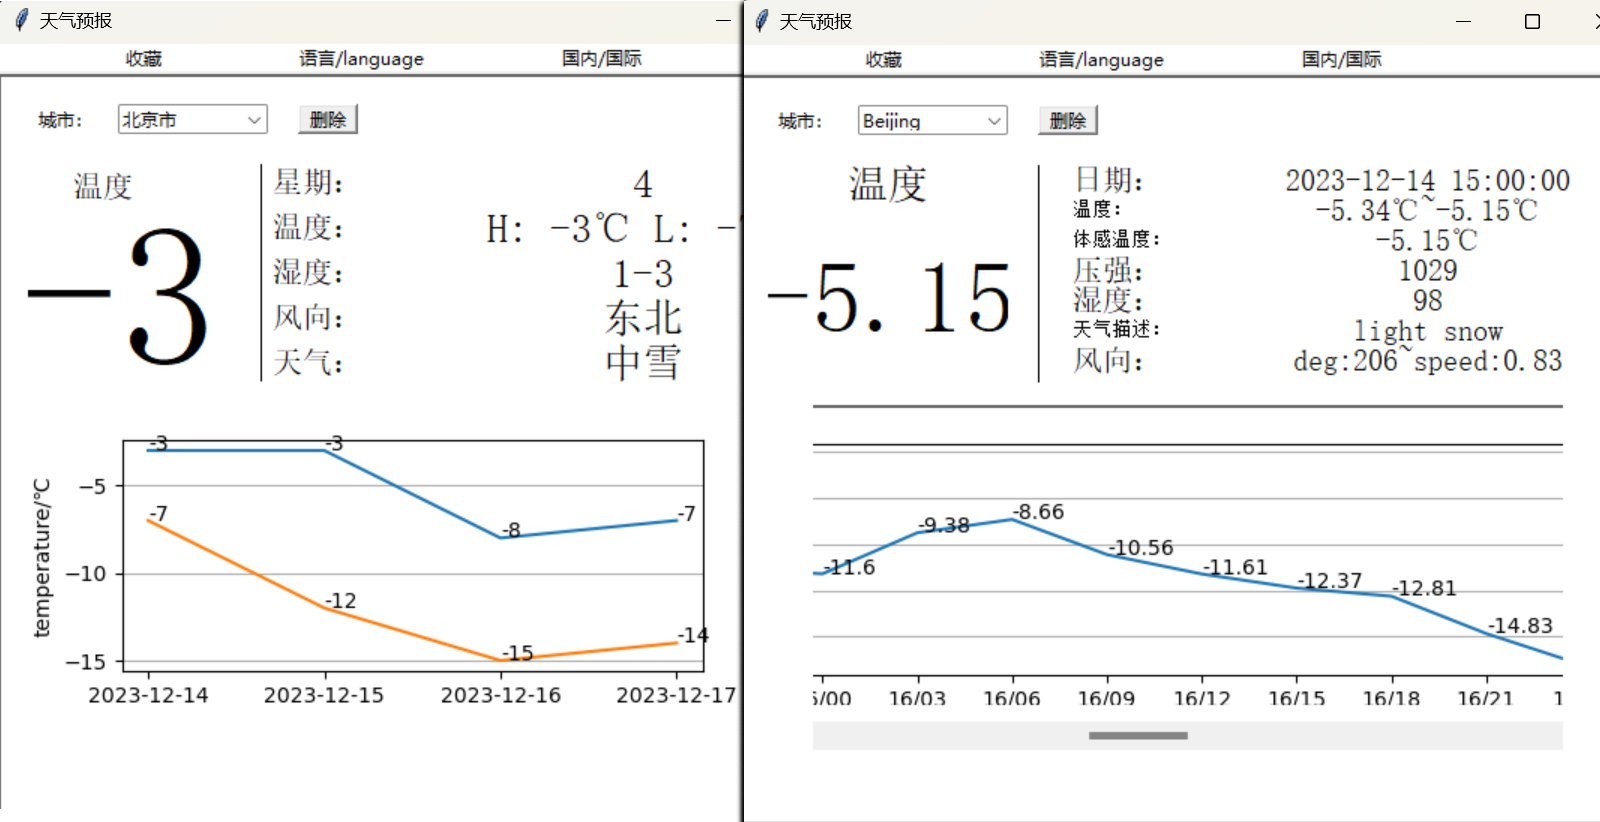
\includegraphics[width=0.8\textwidth]{picb4.png}
               \caption{收藏列表}
            \end{figure}
         \end{itemize}
   \item 语言切换:
         \begin{itemize}
            \item 用户可以通过切换语言按钮选择中文或英文。
            \item 应用根据选择切换显示语言。
         \end{itemize}
         \begin{figure}[H]
            \centering
            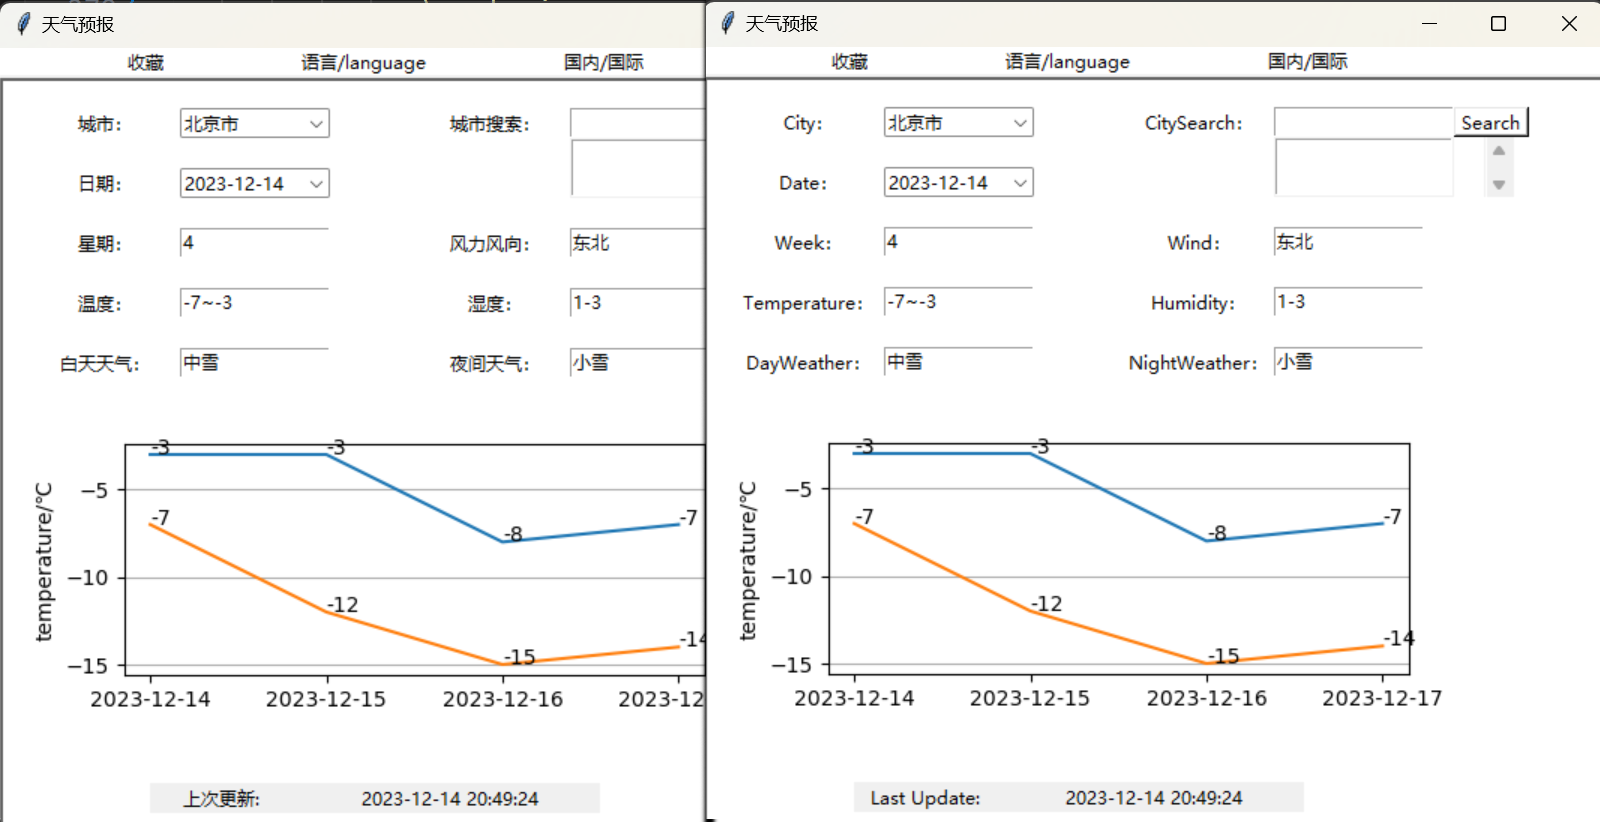
\includegraphics[width=0.8\textwidth]{picb5.png}
            \caption{语言切换}
         \end{figure}
\end{enumerate}

\section{总结与体会}
\begin{itemize}
   \item 通过本次实验,我学会了如何使用requests库调用API接口获取天气信息,如何使用tkinter库创建图形用户界面,如何使用matplotlib库绘制天气趋势图。
   \item 我将课上学到的知识用到了实践上,对数据类型,类,图形界面等有了更加深刻的认识。
   \item 从写完第一版到最终版,我从一个程序员的角度考虑复用性、可读性、可维护性等问题,对代码进行了多次重构,使得代码更加简洁、高效。
   \item 在实验中,我遇到了很多问题,如如何将API返回的JSON数据转化为对象,如何将天气信息嵌入到图形界面中,如何实现数据的持久化等等。
         通过查阅资料,我一一解决了这些问题,对Python的使用更加熟练。
   \item 最后,感谢老师和助教平时的教导和解惑,让我对python的掌握更深了一些。
\end{itemize}


\end{document}